%
% Document template suitable for use as a latex master-file for masters
% thesis in University of Turku Department of Information Technology. 
% Relies on itpackage.sty for additional definitions.
%
% Sami Nuuttila (samnuutt@utu.fi) 
%
% Last mod 2.9.2015:
%
%%%%%%%%%%%%%%%%%%%%%%%%%%%%%%%%%%%%%%%%%%%%%%%%%%%%%%%%%%%%%%%%%%%%%%%%%%%
%
% load all required packages
%
%%%%%%%%%%%%%%%%%%%%%%%%%%%%%%%%%%%%%%%%%%%%%%%%%%%%%%%%%%%%%%%%%%%%%%%%%%%

% document is based on report class
\documentclass[a4paper,12pt]{report}

% load ams-packages for maths
\usepackage{amssymb,amsthm,amsmath}

% load url package for urls, specifically in references
% Use hyphenation
\usepackage[hyphens]{url}
\usepackage{hyperref}

% JH: modified latin to UTF-8 encoding cues to make Scandinavian characters works
\usepackage[utf8]{inputenc}
% load babel-package for automatic hyphenation
\usepackage[english]{babel}

\usepackage{ifpdf}
\usepackage{graphicx}

% Allows for full text citations
\usepackage{bibentry}

% load tocbibind package 
%   - do not include table of contents in itself
%   - convert the name of bibliography to references
\usepackage[nottoc]{tocbibind}

% load sverb package
%   - enhanced handling of verbatim stuff; listing environment
\usepackage{sverb}

% load listings package
%   - handle inclusion of source code
% Use listings-rust from ./thesis/listings-rust.sty
\usepackage{listings}
\usepackage{thesis/listings-rust}

\lstdefinestyle{mystyle}{
  numberstyle=\tiny,
  basicstyle=\ttfamily\small,
  keywordstyle=\bold,
  breakatwhitespace=false,
  breaklines=true,
  keepspaces=true,
  showstringspaces=false,
  showtabs=false,
  tabsize=2
}

\lstset{style=mystyle}

% load fancyheaders package
%   - the actual headers and footers are set later
\usepackage{fancyhdr}

% load itpackage 
%   - additional defines and stuff
\usepackage{thesis/itpackage}

\usepackage{hyperref}

% \lstset{language=Rust, style=boxed}
\lstset{basicstyle=\tiny,style=mystyle}

% uncomment the following snippet to get rid of Luku/Chapter text at the
% beginning of each Chapter... 
%\makeatletter
%\renewcommand{\@chapapp}{\relax}
%\renewcommand{\@makechapterhead}[1]{%
%  \vspace*{50\p@}%
%  {\parindent \z@ \raggedright \normalfont
%    \ifnum \c@secnumdepth >\m@ne
%        \huge\bfseries \@chapapp\space \thechapter\space\space
%    \fi
%    \interlinepenalty\@M
%    \Huge \bfseries #1\par\nobreak
%    \vskip 40\p@
%  }}
%\makeatother

\begin{document}

\selectlanguage{english}

% Set some names based on selected language; no modification required
\settocbibname{References}
\renewcommand{\appname}{Appendices}

% Fill in your information below
\workinfo{Jani Anttonen}
{Proof of Latency Using a Verifiable Delay Function}
{Jaakko Järvi}
{Najmul Islam}
{2021}
{May}
{Toukokuu}

% Set the type of your thesis (Diplomityö, TkK -tutkielma, etc.) and
% laboratory or field of study below
\worktype{Master's Thesis}{M.Sc.}
\deptinfo{Department of Future Technologies}

% Generate the title page 
\gentitle

% Include the abstract
% \begin{ittiivis}{tähän, lista, avainsanoista}
Tarkempia ohjeita tiivistelmäsivun laadintaan läytyy opiskelijan
yleisoppaasta, josta alla lyhyt katkelma.

Bibliografisten tietojen jälkeen kirjoitetaan varsinainen tiivistelmä.
Sen on oletettava, että lukijalla on yleiset tiedot aiheesta.
Tiivistelmän tulee olla ymmärrettävissä ilman tarvetta perehtyä koko
tutkielmaan. Se on kirjoitettava täydellisinä virkkeinä,
väliotsakeluettelona. On käytettävä vakiintuneita termejä. Viittauksia
ja lainauksia tiivistelmään ei saa sisällyttää, eikä myäskään tietoja
tai väitteitä, jotka eivät sisälly itse tutkimukseen. Tiivistelmän on
oltava mahdollisimman ytimekäs n. 120 -- 250 sanan pituinen itsenäinen
kokonaisuus, joka mahtuu ykkäsvälillä kirjoitettuna vaivatta
tiivistelmäsivulle. Tiivistelmässä tulisi ilmetä mm.  tutkielman aihe
tutkimuksen kohde, populaatio, alue ja tarkoitus käytetyt
tutkimusmenetelmät (mikäli tutkimus on luonteeltaan teoreettinen ja
tiettyyn kirjalliseen materiaaliin, on mainittava tärkeimmät
lähdeteokset; mikäli on luonteeltaan empiirinen, on mainittava käytetyt
metodit) keskeiset tutkimustulokset tulosten perusteella tehdyt
päätelmät ja toimenpidesuositukset asiasanat
\end{ittiivis}

% if your thesis is in english then this is also required (is it???)
%\begin{itabstract}{list, of, keywords}
%If your thesis is in english this might also be required???
%\end{itabstract} BROKEN ATM

% empty pagestyle for table of contents etc. 
%
% the redefinition of plain style works also for 1st pages of chapters,
% which is the default in report class. Just state \thispagestyle{empty}
% after \chapter{something} if you want empty style for the 1st pages. 
%
\pagestyle{empty}
\fancypagestyle{plain}{
	\fancyhf{}
	\renewcommand{\headrulewidth}{0 pt}
}

% roman numbering for table of contents etc.
\pagenumbering{roman}

% insert table of contents, list of figures, list of tables
%
% setting the counter to zero effectively removes the page number from
% the toc, lof etc. entries in the toc since there is no roman numeral
% for zero ;-) (if you want them without numbering)
%
%\setcounter{page}{0}
\tableofcontents
\clearpage
\setcounter{page}{0}
\listoffigures
\clearpage
\setcounter{page}{0}
\lstlistoflistings

% possibly insert 'list of acronyms'
%
%   - create a chapter called List Of Acronyms (or whatever), which
%     should contain all your acronym definitions, e.g. 
%     \chapter{List Of Acronyms} 
%   - the secnumdepth trickery is needed because acronyms are as a
%     standard chapter and we are faking '\listofacronyms'
%
%\setcounter{secnumdepth}{-1}
%% !TeX root = ./Terms.tex
\section*{Käsitteet}
\begin{description}
	\item[BASE] \hfill 
			
	\textbf{Basically Available} -- Jokaiseen kyselyyn vastataan, palautusarvolla ei väliä.
	\item[Ebin] \hfill
	ebon 
\end{description}

%\setcounter{secnumdepth}{2}

% setup page numbering, page counter, etc.
\startpages

%%%%%%%%%%%%%%%%%%%%%%%%%%%%%%%%%%%%%%%%%%%%%%%%%%%%%%%%%%%%%%%%%%%%%%%%%%%
%
% Thesis starts here. Create a new tex file for each chapter and input it below. You may encounter errors if you use å, ä, ö or <space> characters in referred names.
%
% Good luck!
%
%%%%%%%%%%%%%%%%%%%%%%%%%%%%%%%%%%%%%%%%%%%%%%%%%%%%%%%%%%%%%%%%%%%%%%%%%%%

% !TeX root = ./Thesis.tex
\chapter{Introduction}
\label{Introduction}

Computer applications, whether they are on the public Internet or on a private network, commonly use the client-server model of communication. In this model, the client application sends requests to the server, and the server responds. Applications are today, however, increasingly moving towards a distributed, peer-to-peer (P2P) networked model, where every peer, whether it is an entire computer or merely a process running on one, serves equally as the both sides of the client-server model. Many uses of P2P are not visible to the end user, because in many cases, P2P technologies serve to optimize resource utilization rather than as centerpoints of applications. For example, the music subscription service Spotify's protocol has been designed to combine server and P2P streaming to decrease the load on Spotify's servers and save bandwith, and thus improve the service's scalability.~\cite{Kreitz_undated-yp} Naturally, P2P streaming comes in handy also whenever there is a short outage, as users might not experience any stoppages to the service, at least when listening to widely streamed content. 

The aspects of peer-to-peer networking that have recently gotten attention are cryptocurrency and blockchain technologies, categorized under the roof term of distributed ledger technologies. Prior to the emergence of ledger technologies, peer-to-peer systems were often seen in the public light as a technology to work around regulations and for doing lawless activities. This is partly because before their use in blockchain applications, P2P systems were popularized for their use in file sharing applications like Bittorrent. Obviously, this reputation was not earned for nothing, but peer-to-peer networking's use in torrents and other file sharing networks also demonstrates its potential in content delivery networks, or CDNs for short. Peer-to-peer networks are not without problems. One persistent source of problems is routing and peer discovery. Since the users of a P2P network do not necessarily connect to a centralized and optimized server infrastructure with vast bandwidth and computation resources, the individual connections between peers can be ephemeral, and routes between peers that are not directly connected are usually random. This results in some routes between peers to be inoptimal, which could result in bad performance and even false states in distributed ledgers, where slow data propagation in a P2P publish-subscribe network could mean inability to participate in the consensus due to latency. % AND THEN WHAT yes, describe the problem

Blockchain networks need a way of synchronizing the latest state of the blockchain globally between a number of peers on a P2P network. Since the blockchain data model is sequential and all recorded history is immutable, an algorithm is needed to reach total synchronization and agreement between peers. This kind of an algorithm is called a consensus algorithm. Consensus problems are not unique to blockchains, but are also relevant in distributed databases. Blockchains have raised new issues in consensus algorithms that have sparked an ongoing development effort for new kinds of consensus algorithms.

Proof of Work is the most used consensus algorithm in public blockchains today, including in Bitcoin, where it was first described in 2008.~\cite{Nakamoto2019-ax} In short, in Proof of Work all participants try to guess a correct answer to a cryptographic puzzle as fast as they can, and a correct answer produces a new block. The new block gets sent and propagated to the network, and if enough peers agree that the answer was correct, the guessing game starts over. In Proof of Work, any latency at all results in wasted resources for all participants before they receive the latest block, as they are still trying to solve the puzzle before they know the result.

As latency is not only a physical and a computational problem in P2P networks, but rather an algorithmic one, search for alrorithmic solutions has long been a part of P2P networks research. Since latency between peers in P2P networks is a problem of the network topology, the solutions have tried to optimize the peer discovery mechanisms. This has worked to some degree, with randomized peer discovery and a high amount of concurrent connections resulting in P2P networks with good peer discoverability and resource availability, but with subpar routes between peers that are not directly connected to each other.

If a peer told you its individual latencies to other peers on its routing table, couldn't this help with constructing an optimal distributed routing table, with peers only connecting to other peers if they are actually close-by or behind a fast connection? I think that it could, but since only a certain number of connections can be kept at one time, this would increase the possibility for so-called eclipse attacks. In an eclipse attack, an attacker tries to influence the victim's connections in a way that it would only be connected to peers controlled by the attacker, effectively isolating the victim from honest peers on the network, increasing the possibility for man-in-the-middle attacks regarding the victim's sent requests or received responses. Also, a not-so-malicious peer could try to game the peer discovery algorithm in the pursuit of better connections to itself at the cost of others. Whilst this is not as severe of a problem, it's still undesirable.

Now, what if you didn't have to trust the peer who reports the latencies, but instead there was no way for the other peer to lie on the subject? Given these tools, a peer could roughly estimate the network topology and find the peers closest to it with a roughly optimal amount of queries, and the P2P network could converge towards an optimal topology with limited threat of eclipse attacks. Such a proof of latency could also be used to prove a geographical location, which could be used to battle GPS spoofing. 

% TODO: Siirrä tästä eteenpäin olevat jutut backgroundiin / VDF:iä koskeviin kappaleisiin
Many other algorithms have been introduced for achieving consensus in blockchains. In Proof of Stake network nodes participate in the voting of new blocks by staking a part of their assets as a pawn. Concretely this means that a peer hands the control of some of its cryptocurrency to the consensus algorithm. If a voter gets labeled as malicious, faulty, or absent by a certain majority, its stake can get slashed, losing all or a part of the staked asset in the process. This serves as an incentive for honest co-operation, with sufficient computation resources.

One problem with Proof of Stake is that the block generation votes are not done globally, but by a selected group of peers called the validators, which vote for the contents of proposed blocks that are generated by just one peer at a time, selected as the block generator. The validators are usually selected randomly. This has generated an increasing demand for verifiable public randomness that is pre-image resistant, meaning the output of the algorithm generating the randomness cannot be influenced before evaluation by input. This created a need for an algorithm that would prevent multiple malicious actors from being selected to vote at once. A cure for this problem is called a verifiable delay function, a VDF in short. Verifiable delay functions can help in creation of public randomness simply because they produce quickly verifiable proofs for results that have high entropy due to repeated calculations with a pre-image resistant hash function. The hash function inside a VDF can be changed, and VDFs' use in such distributed random beacons is only a small piece of a larger puzzle, as good randomness is hard to achieve using only pseudo-random hash functions. Another problem which served as a motivation to find such a function is scalability and data integrity in distributed ledgers. If the participants of a distributed network of nodes have the same initial input for a high-frequency hash function, and they have similar hardware, it can help putting transactions in order without explicit communication between peers, since you can index each transaction with a hash before communicating it to other peers. The resulting order can be incorrect, but like the case with other forms of synchronized distributed clocks, the main objective is to have an explicit order without ambiguity. This also ties into CRDTs\footnote{Conflict-free Replicated Data Type}, but since that is not the main subject of the thesis, I will not address it.

Time-lock puzzles are precursors to VDFs. Their evaluation can be similar or even identical, but they do not contain a proof that is faster to calculate than to re-evaluate the whole puzzle. One example of such proof would be to link each iteration of the puzzle's evaluation to the previous iteration, and supply each step of the calculation to the proof's verifier. Then the verifier can use parallel computation to verify the proof faster than re-evaluating the whole thing. A proof of this sort is categorized as being a proto-VDF, since there are better and more bandwidth-efficient ways to construct a VDF proof, and some could argue the proof is not strictly a calculated one.

In 2018, two research papers were released independently with similar formalizations of a VDF.~\cite{Wesolowski2018-rf, Pietrzak2018-xs} VDF is an algorithm that requires a specified number of sequential steps to evaluate, but produces a proof that can be efficiently and publicly verified.~\cite{Boneh_undated-ml} To achieve pre-image resistance, a VDF is sequential in nature, and cannot be sped up by parallel processing. There are multiple formulations of a VDF, and not all even have a generated proof, instead using parallel processing with graphics processors to check that the delay function has been calculated correctly.~\cite{Yakovenko2018-zn} This bars less powerful devices, like embedded devices, from verifying the VDF's result efficiently. Thus, generating a proof that requires little time to verify is more ideal.~\cite{Boneh_undated-ml}

VDFs could see usage in many things not directly related to blockchains or distributed ledger technologies, and my motivation for this thesis is to find such new use cases. I believe I have found one that is somewhat related to the distributed synchronized clock mentioned earlier, using a similar parallel construct between two peers to measure latency with iterations of a sequential computation.
% TODO: Tähän saakka tulevat jutut backgroundiin

% TODO: Elaborate on eclipse attacks, add citations on the matter
Using a verifiable delay function, I propose a novel algorithm for producing a publicly verifiable proof of network latency and difference in computation resources between two participants in a peer-to-peer network. This proof can be used for dynamic routing to achieve better, faster routes between peers, and for making eclipse attacks\footnote{Eclipse attack means polluting the target's routing table restricting the target's access to the rest of the network, which opens up other attack possibilities regarding consensus algorithms.} harder to achieve. 

% !TeX root = ./Thesis.tex
\section{Cryptography}

Cryptography is a field of mathematics that uses computationally difficult problems to obfuscate, hide, split and verify data. Starting in the ancient times with the famous Caesar cipher, which relied on shifting the letters in a message in coordination to an alphabet, there are multiple cryptographic protocols today for a variety of use cases, which are used in both public and private messaging. As mentioned earlier, while the familiar connotation of cryptography as a word brings secrecy and secure communications into mind, it can also be used to verify data, and to prove that something has happened. I will go over cryptography subjects that are relevant to the Proof of Latency protocol in this chapter, like groups of unknown order, RSA and cryptographic proofs.

Modern cryptography is based on relatively few mathematical fundamentals. The most dominant one during the age of computers has been prime numbers with modular multiplication, but elliptic curve cryptography is used widely today because of its easy and less resource-intensive key generation method when compared to the prime number based RSA cryptosystem. They both use modular arithmetic in their operations.

Modular\footnote{Using the modulus operation; taking the remainder of a division. Useful in cryptography because it creates finite cyclical groups.} arithmetic with large numbers has a useful property that you can exchange encrypted data without the participants knowing each other's private keys, but requiring a computation that is theoretically almost impossible to break due to the prime factorization problem. These large numbers that are used as the modulo need to have unknown factorizations to create groups of unknown order, that are paramount to cryptographic systems that rely on the factorization problem for their safety. The order of a group means the amount of elements in it. Cryptographic proofs need to be created with groups of unknown orders for them to be valid, as knowing the order of a group means that the modulo used in the cryptographic operations is so small that it has a known factorization, and the security of the factorization problem is broken.

\subsection{RSA}
RSA is named after it's discoverers – Rivest, Shamir, Adleman. It is an asymmetric public-key cryptosystem, meaning that it is based on a keypair, in which one is a public and the other is a secret. The public key is used to encrypt, and the secret key is used to decrypt. Everyone who has the public key can encrypt data and that encrypted data is practically impossible to decrypt without the secret key. This works due to the fact that it is hard to factor the product of two large prime numbers. RSA has been the most widely used cryptosystem since its creation, and is easy to use in modern context by just increasing the size of the keys.

RSA is an arithmetic trick that creates a mathematical object called a trapdoor permutation. Trapdoor permutation is a function that transforms a number x to a number y in the same range, in a way that computing y from x is easy using the public key but computing x from y is practically impossible without knowing the private key. The private key is the trapdoor.~\cite{Aumasson2018-nh} RSA relies on the prime factorization problem and the strong RSA assumption for its security. Strong RSA groups are groups of unknown order, meaning that the number of elements in the group is unknown. RSA has played a big part in the development of cryptography, and even served as a motivation for the creation of verifiable delay functions, as it was used in the creation of time-lock puzzles closely related to VDFs.
% TODO: Not the correct assumptions listed here

\subsubsection{Setup}
At first, the users need to setup the public parameters, which need to be distributed between the involved peers to be used in encryption. This key generation process is quite resource intensive, and is rarely used in ephemeral contexts, unless you can skip the key generation process, or ceremony, and use a publicly available modulo that is created by a trusted party. These types of key generation processes are called trusted setups, and they produce so-called toxic waste that needs to be discarded to preserve the key safety.

The company formed by the RSA algorithm's inventors, RSA Security LLC, published public RSA semiprimes\footnote{A product of two prime numbers} that are called RSA numbers as a part of the RSA factoring challenge from 1991 up until 2007 when the challenge ended.~\cite{RSA_Laboratories2013-zk} The challenge was ended because it had reached its purpose of forwarding science and understanding of common symmetric-key and public-key algorithms. Despite this, still under a half of the RSA numbers have been factored, and the largest of them might take hundreds if not even thousands of years to break even when given extraordinary hardware to do it with.

Using these factoring challenge RSA numbers requires the user to assume that nobody has access to the parameters. Given that the RSA numbers are said to have been created with a machine that was completely destroyed after their creation and the primes were never apparent to anyone, you need to trust the company's claims if you ever use these public challenge numbers. Fortunately, usually they are not used for encrypting large swathes of personal data, but in a more ephemeral context like Proof of Latency, which wouldn't cause a huge stir if the cryptosystem was broken and needed changing.

\subsection{Cryptographic Proofs and Their Soundness}
Cryptographic proofs are proofs that depend on the trapdoor nature of cryptographic functions. In other words, cryptographic proofs are arguments that can be trusted if the cryptographic assumptions they depend on are valid and not broken. The most well-known proofs, which are not necessarily thought of as such, are digital signatures. Given a public key, a prover in possession of its corresponding private key can produce a signature of any given data, given to a verifier together with the original data that the prover has seen and processed the data. If the private key pertaining to the public key gets leaked to a third party, its security is broken, and the unique identity is lost.

Proofs can be private or public. A cryptographic proof can be categorized as public, if a verifier can gather all information required to verify the proof from the transcript of the proof itself, and verify the proof to be correct. Now, since classical cryptography is based on the fact that a computation is asymmetric --- being harder to compute the other way around, a cryptographic proof is still probabilistic in nature, and the security of it based not only on the algorithm but also the parameters used.

Proofs need to be tested for soundness to be called as such. Soundness means that a prover cannot make a verifier accept a false statement with reasonable probability. This means that a proof is dependent on context, the verifier. If a proof holds statistically, it's a proof. If it instead holds only computationally, it should be instead called an argument.


\subsection{Commitment Schemes}
Commitment schemes are a way to lock causality in a cryptographic protocol, an are among the most used primitives in cryptography. Commitments usually come in the form of commit-reveal, when at a later stage of the protocol the committee reveals the original value \(x\) they made their commitment \(C\) on. This has a great property --- a prover cannot change their committed value after revealing their commitment to the verifier, because the commitment would not hold for a new value. Commitment schemes are usually used when an interactive protocol requires for a value to be hidden until the termination of the protocol.

\subsubsection{Vector Commitments}
Vector commitments are a recently formalized primitive consisting of a vector \(V\) that as you guessed it, is filled with commitments. The simplest form of a vector commitment most already know is a merkle tree. Unfortunately, merkle proof size grows with input, but newer forms of vector commitments have been discovered after its formalization in 2013. For example, Catalano-Fiore vector commitments improve upon the proof size, introducing a fixed size proof. In addition to the fixed size, the verifier only needs to know the proof and the digest, or the latest output, to verify the proof. In layman's terms, vector commitments enable a prover to prove that a commitment \(v_n\) has been made at the index \(n\) of vector \(v\).

%TODO: Add a formal definition of vector commitments and regular commitments (use an example like Pedersen commitments)

Like regular commitment schemes, vector commitments are used to enforce causality. While regular commitment schemes make sure that a user of a protocol can't change an input or "skip the line" after the start, vector commitments create a causal relationship for multiple proofs. To wrap it up, if proofs are based on vector commitments, the commitments guarantee that the proofs' order can't change, unless the whole vector with all associated proofs are unvalidated.

A Merkle tree is a data structure and a cryptographic accumulator in which you can traverse to the tree's root from any leaf node on it, as a node is always linked to the previous node by a hash that has been calculated with the hash of the previous node. That's right, a blockchain is a Merkle tree, but with added steps.


% !TeX root = ./Thesis.tex
\chapter{Peer-to-Peer Networking}
\label{Peer-to-Peer Networking}
Peer-to-peer networking, P2P in short, means that two or more devices communicate with each other with both serving as a client and a server simultaneously. P2P networks vary in scope a lot. Some networks are global, while some are as small as a couple of devices in a local area network, which is the case in printer sharing and some IoT installations. P2P networks can be standalone or rely on some existing infrastructure, like the internet. The P2P networks that rely on preexisting infrastructure are called overlay networks.

While overlay networks' addressing and routing is usually based on TCP/IP or UDP/IP, they must introduce a separate routing scheme, like a DHT, that works as an index for peers on the network. Since IP only focuses on addressing the computers and not the applications or resources they offer, it can't function as a peer discovery scheme by itself.

Overlay P2P networks must somehow signal the initial peers, also called bootstrap or introductory peers, to connect to at first. This can be done either by including the bootstrap peers' IP addresses in the application code itself or by providing the same information on a regular web page. The bootstrap peers can be also signaled by word-of-mouth between a group of people, or with wireless broadcast, which I will touch a bit on the next section. This said, usually every peer can function as a bootstrap peer, so knowing the connection info of a single peer on the network can potentially introduce you into the network at large.

A simple way to create a P2P network would be to share a single file with anyone who connects to you that has all the IP addresses you've ever connected with. This would be an example of an unstructured P2P network, which could work relatively well in a closed setting, like inside a LAN if there's no support for multicast DNS, or mDNS in short.

\begin{figure}
	\includegraphics[width=\textwidth]{pictures/unstructured.png}
	\caption{Example topography of an unstructured overlay network}
	\label{Unstructured Overlay Network}
\end{figure}

In contrast to unstructured networks, where peers are connected to at random, structured networks have some logic that is used to form a structured overlay network rather than just connecting to peers as they come.

\begin{figure}
	\includegraphics[width=\textwidth]{pictures/structured.png}
	\caption{Example topography of a structured overlay network}
	\label{Structured Overlay Network}
\end{figure}

\section{Ad Hoc and Zero Configuration Networking}
Multicast DNS was proposed by Apple in 2013~\cite{Cheshire2013-ja} as a way of discovering peers in a local area network in a zero-configuration manner. It is used today for resource sharing, such as sharing printers. Multicast DNS does not work outside local area networks, since it works by associating names with IP addresses like regular DNS does. The problem is that these names are not quaranteed to be unique, and therefore can be spoofed. If there are two clients with the same name, the first one to respond with its IP address to a query wins.~\cite{Pdp2008-tg} The security of zero-configuration and ad hoc networking must relay on cryptographic identities, so that a peer can verify itself with public-key cryptography, that makes the peers on the network practically unique and thus hard to spoof.

% TODO: Seuraavaksi väite, cite!
Zero-configuration networking in an unconstrained, global setting is possible with radios, using either dedicated meshnet radios like GoTenna~\cite{GoTenna_undated-km} or Helium~\cite{Helium_undated-jv}, or by using the antennas inside mobile devices to form a network. These types of networks are usually called meshnets or ad hoc networks. Basically, Walkie-Talkies are the simplest form of a P2P network. Problems can arise due to geography blocking signals, or when you want to cross large distances with the transmitting capability of a pocket device. Mesh networking has been used most famously in protests worldwide by using a smartphone app called Firechat.~\cite{Milian2014-mt}

Ad hoc mesh networks have a natural metric for latency, signal strength. They can rely on Bluetooth RSSI\footnote{Received Signal Strength Indication}, or triangulate distances by cooperating with multiple peers. These methods are used to locate emergency calls, and in contact tracing.~\cite{Biddle2020-kl} Mesh networks, while being peer to peer and not relying on existing infrastructure like overlay networks, still need routing and multiple hops if one wants to reach peers that are not in the operating range of the communication method used. Even ad hoc networks could benefit from having a Proof of Latency, although the proofs should be updated way more frequently because of their mobile nature.

\section{Distributed Hash Tables}
Distributed hash tables are a way of pointing content to peers in a distributed network. In addition to indexing content in content-addressed networks like IPFS~\cite{Labs_undated-uw}, they can function as routing tables, and have been developed to remove bottlenecks in peer search. A hash table is a key-value mapping from a to b. What makes them distributed is the fact that the data stored is meant to be distributed between peers, with not a single peer keeping all the available data in its hash table, but relaying queries for resources it does not have to other peers on the network. There are multiple versions of DHTs with different methods for prioritizing certain peers, using tree structures, sorting by identifiers, using computational trust et cetera.

In addition to identifier closeness, DHTs can force a certain network behavior by peer scoring and constructing a web of trust. For example, a peer could only advertise peers that have been connected over a period of time, or enforce reconnecting to disconnected peers that have a good reputation. Computational trust is bayesian in nature, optimizing a single value over time, and simulating remembrance and forgettance. A widely used trust system like this is TrustGuard, implemented in the blockchain framework Tendermint.~\cite{Srivatsa2005-ib, Jeff_Foley2018-zt}

Most of the DHT algorithms were invented in the early 2000s, with Kademlia being one of them. DHTs mostly differ just by how distance is defined, and how the neighbors are chosen.~\cite{Cai2015-ra}

\subsection{Kademlia}
Kademlia is a DHT designed by Petar Maymounkov and David Mazières in 2002. It is based on a tree of identifiers which are split across peers on a network. The identifiers are 160 bits, e.g. a SHA-1 hash of some larger data. Kademlia tries to improve upon previous DHT-based routing algorithms by introducing a symmetric XOR metric for distance between node IDs in the key space.~\cite{Petar_Maymounkov2020-sx} These IDs are sorted in a binary search tree, with each node's position determined by the shortest unique prefix of its ID, like shown in diagram \ref{Structured Overlay Network} on page \pageref{Structured Overlay Network}. Kademlia makes sure that any node in the network can locate any other node by its ID by making sure that each node knows at least one of the nodes in each subtree.

A single query in Kademlia has been shown in real-world tests to result in an average of 3 network hops, meaning that the query gets relayed through two peers before reaching the requested resource.~\cite{Roos2013-mb} Network hops are a necessary evil in distributed systems, and Kademlia does well in requiring on average a log(n) queries in a network of n nodes. Since the closeness metric is based on a similarity search rather than a measurement, the closest peer is only closest by the identifier, not by network latency.~\cite{Eigenmann2020-zm}

The randomness of Kademlia is great at averaging the network hops required to reach a scarce resource. The downside is that it also averages everything else, increasing latency to closest connected peers, reducing overall performance of the network.

Kademlia protocol has four remote procedure calls, or RPCs in short. These are PING, STORE, FIND\_NODE, and FIND\_VALUE. A Kademlia participant's most important operation is node lookup, which is locating k closest nodes to a given node ID. It is a recursive operation, which starts by picking alpha closest nodes from its closest non-empty bucket, and sending them all FIND\_NODE calls. This is repeated until the initiator has queried and got responses from all k closest nodes it has seen.

\section{Eclipse Attacks}
Although Kademlia is most widely used with random hashed identifiers, the distance metric stays the same. By forging identities that are close-by, you can advertise false friends which take over the search space. For example, in a 2019 paper "Eclipsing Ethereum Peers with False Friends" by S. Henningsen, D. Teunis, M. Florian, and B. Scheuermann, they demonstrate that to eclipse a victim in Ethereum P2P network, you need to fill its 8 slots for outbound connections, and fill 17 slots for inbound connections to completely deny service without going through the attacker's nodes.~\cite{Henningsen2019-mf}

Less structured, random ways of forming connections in an overlay network, like Kademlia, protect against eclipse attacks quite well because of the high connectivity and low locality. Introducing peer scoring and making the network topology more structured opens up possibilities for an attacker to game the scoring system, making sure the target connects to lots of sybil peers eclipsing it. Thus, protecting against eclipse attacks is a balancing act that requires an overlay network to retain some elements of an unstructured network while improving general performance with a structured group of peers.~\cite{Mao2020-ee} This balancing act is seen as a multi-armed bandit problem of exploration and exploitation in the 2020 paper "Perigee: Efficient Peer-to-Peer Network Design for Blockchains" by Y. Mao, S. Deb, S.B. Venkatakrishnan, S. Kannan, and K. Srinivasan.


% TODO: More stuff here

% !TeX root = ./Thesis.tex
\chapter{Verifiable Delay Functions}
\label{Verifiable Delay Functions}

\section{Applications}

\section{Variations}

\section{Similar Constructs}
A VDF can only be calculated sequentially, but even without a proof there is a possibility to make the verification faster through parallellism.\cite{yakovenko_solana_nodate} 


% !TeX root = ../Thesis.tex
\chapter{Proof of Latency}
\label{Proof of Latency}
Proof of Latency, "the algorithm" or "PoL", is a collection of two algorithms that when used in a P2P context, can offer a robust way of reducing network latency between peers on the network by minimizing the number of hops between peers that are close in terms of performance and geographical location.

The first version of the algorithm requires a trusted setting, preferably a trusted computing platform from all participating peers, while the second version is trustless and requires no specific hardware from the participants, while a trusted computing platform would make it fairer and more reliable, by not discriminating based on CPU performance.
\section{Role of Latency in Distributed Systems}
It's hardly a surprise, but latency is a huge factor in distributed systems, especially trustless, decentralized ones. Latency is mostly constrained by the speed of light, which can not be changed, and thus there are concrete factors that must be taken into account when designing a p2p system with routing. In 2012, the global average round-trip delay time to Google's servers was around 100ms.\cite{grigorik_latency_nodate}

In the new space age the maximum possible latency grows very fast, as there could be peers joining to a distributed network from other planets, space ships or stations. This might be unnecessary to think about in the distributed P2P context for now, but before all that, we have global satellite mesh internet providers, like Starlink. Elon Musk, the founder of SpaceX, which provides the network of satellites, claims that there's going to be a latency of about 20 milliseconds.\cite{tung_elon_nodate} But, since speed of light restricts us to about 100ms of minimum global latency\cite{noauthor_satellite_nodate}, those claims cannot be trusted. In legacy satellite internet access, the round-trip time even in perfect conditions is about 550 milliseconds.\cite{noauthor_satellite_nodate}

\section{Network Hops Increase Latency}
Network hops in P2P systems are introduced when two peers are not directly connected to each other, but rather through one or many relays. There are network hops that cannot be easily avoided, like the hops between network routers in the internet already. Most of the P2P routing protocols used today are oblivious to the problem of introducing large hops to communications between two peers. These DHT-based protocols, like Kademlia, make the assumption that their users have fast internet access, and minimize the average latency by selecting connected peers basically at random.

While the randomness is great for preventing eclipse attacks, they can introduce unnecessary geographical hops between two peers. If two peers are in the same WAN, for example, in Kademlia they might still connect to each other through a network hop going through another continent. This makes individual connections less efficient.
Now, if we were to rely on IP address geolocation, we could more efficiently connect to peers that are close-by. This is unfortunately impossible in privacy-oriented P2P networks, like mixnets, which aim to hide as much of the packet routing information as possible, by routing individual packets through different peers and hiding IP addresses of two connected peers from each other.\cite{nym_sphinx_2020}

Proof of Latency is made to improve the performance of current P2P networking solutions and make them future-proof, even for hops between planets, while still being compatible with some privacy-preserving P2P protocols.

\section{First Version of PoL}
The first iteration of the algorithm is based on an attempt to simplify the initial Proof of Latency algorithm. After some thought, I came to the conclusion that the initial iteration, which ended up as the second and final version of the algorithm, is actually the most resistant to attacks and requires less trust from the participants.
\begin{figure}
	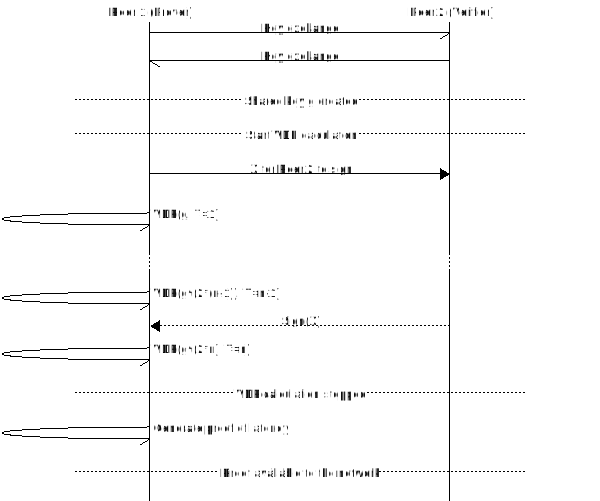
\includegraphics[width=\textwidth]{pictures/pol_diagram.eps}
	\caption{Protocol diagram of Proof of Latency}
	\label{Diagram 1}
\end{figure}

\subsection{Results}
Since the network peers are trying to compete with each other for the least latency, they win the game by calculating the least amount of VDF iterations. In the first version of the algorithm, this soon becomes a problem. There's no way to tell how fast another computer is, so in this case spoofed results of 1 iteration would win every time.

This version only works if the peers can trust each other, but in that case we could also resort to using ping. Ways of introducing trust would be using a trusted computing platform, but even that could be vulnerable to undervolting or other physical tampering. This problem drove me to revert back to my original idea, which I'm calling the version two of Proof of Latency.

\section{Second Version of PoL}
The second version of PoL introduces a race between the two peers. Like in the first version, there's a prover and a verifier. The difference here is that they both calculate a VDF and the verifier calculates the difference in iterations between the two.

First they do a Diffie-Hellman key exchange to construct a previously unknown key. Then, they both start calculating a VDF in parallel. The prover only calculates the VDF up to a predefined threshold, and then sends the proof with a signature back to the verifier. The verifier then stops its own calculation, generates a proof of it, and then calculates the absolute difference between the amount of iterations between its own VDF and the prover's.

Since calculating a VDF is relatively easy for modern processors, a VDF over as little as a few milliseconds of time can be a valid way of measuring latency. Still, without an ASIC chip for calculating VDFs faster than any other available processor, these protocols are also a measurement of processing performance. This might introduce an unfortunate barrier for entry for mobile and IoT devices. The second version of PoL is meant to tackle this problem by creating a performance and latency gradient to the network. The network topology results in a gradient that is defined by geographical location and the similarity in performance. This means that connectedness between mobile and IoT devices is going to be better than between devices that have a huge performance difference.

\chapter{Conclusion}
\label{Conclusion}
Since calculating a VDF is relatively easy for modern processors, a VDF over as little as a few milliseconds of time can be a valid way of measuring latency. Still, without an ASIC chip for calculating VDFs faster than any other available processor, these protocols are also a measurement of processing performance. This might introduce an unfortunate barrier for entry for mobile and IoT devices. The second version of PoL is meant to tackle this problem by creating a performance and latency gradient to the network. The network topology results in a gradient that is defined by geographical location and the similarity in performance. This means that connectedness between mobile and IoT devices is going to be better than between devices that have a huge performance difference.


% insert references
%  - included unsrtf.bst provides finnish language version of unsrt
\bibliographystyle{unsrt}
\bibliography{library.bib}

%%%%%%%%%%%%%%%%%%%%%%%%%%%%%%%%%%%%%%%%%%%%%%%%%%%%%%%%%%%%%%%%%%%%%%%%%%%
%
% Almost there....
%
%%%%%%%%%%%%%%%%%%%%%%%%%%%%%%%%%%%%%%%%%%%%%%%%%%%%%%%%%%%%%%%%%%%%%%%%%%%

% make sure pagecount is correct even if references overflow to a new page
\pagebreak\addtocounter{page}{-1}
\eofpages
\appendices

% create your appendix chapters with command \appchapter{some name} instead
% of \chapter{some name} for the automagic page counting to work
%\input{file name of appchapter xxx}
%\input{file name of appchapter yyy}
%\input{file name of appchapter zzz}
%\input{and so on}

%%%%%%%%%%%%%%%%%%%%%%%%%%%%%%%%%%%%%%%%%%%%%%%%%%%%%%%%%%%%%%%%%%%%%%%%%%%
%
% main document ends here
%
%%%%%%%%%%%%%%%%%%%%%%%%%%%%%%%%%%%%%%%%%%%%%%%%%%%%%%%%%%%%%%%%%%%%%%%%%%%
\eofapppages
\end{document}
